\documentclass[8pt,xcolor=table]{beamer}

\usepackage{graphicx}
\usepackage{caption}
\usepackage{subcaption}
\usepackage{transparent}
 
% \usepackage[utf8]{inputenc}
% \usepackage[T1]{fontenc}
\usepackage[table]{xcolor}    % loads also »colortbl« 
%  \usepackage{enumitem}
% \usepackage{ucltemplate}
\usepackage{color}

\usepackage{tabularx} % make width of table columns evenly distributed (see http://tex.stackexchange.com/questions/60601/evenly-distributing-column-widths)
% \newcolumntype{Y}{>{\centering\arraybackslash}X}

% make entire row bold or italic in table
\newcommand\setrow[1]{\gdef\rowmac{#1}#1\ignorespaces}
\newcommand\clearrow{\global\let\rowmac\relax}
\clearrow


\usepackage{amssymb}% http://ctan.org/pkg/amssymb
\usepackage{pifont}% http://ctan.org/pkg/pifont
\newcommand{\cmark}{\ding{51}}%
\newcommand{\xmark}{\ding{55}}%


\usepackage{pgfgantt} % for grantt charts
\usepackage{rotating}
\usepackage[graphicx]{realboxes}
\usepackage[export]{adjustbox}
\usepackage{array}

\usepackage{rotating}
% \usepackage{tabularx, booktabs} % make width of table columns evenly distributed (see http://tex.stackexchange.com/questions/60601/evenly-distributing-column-widths)
% \newcolumntype{Y}{>{\centering\arraybackslash}X}

\DeclareMathOperator*{\argmin}{arg\,min}
\DeclareMathOperator*{\argmax}{arg\,max}

\usepackage{tikz}
\usetikzlibrary{arrows,positioning, shapes.symbols,shapes.callouts,patterns,shapes,chains,calc,backgrounds,fadings}

% \definecolor{parCol}{rgb}{0.1, 0.1, 1}
% \definecolor{stCol}{rgb}{0.1, 0.6, 0.1}
% \definecolor{bothCol}{rgb}{0, 0.5, 0.5}

\definecolor{parCol}{rgb}{0, 0, 0}
\definecolor{stCol}{rgb}{0, 0, 0}
\definecolor{bothCol}{rgb}{0, 0, 0}
\definecolor{blue3}{HTML}{86B7FC} % med blue
\definecolor{blue1}{HTML}{B5F1FF} % light blue
\definecolor{blue2}{HTML}{E0F9FF} % very light blue

\newcolumntype{C}[1]{>{\centering\let\newline\\\arraybackslash\hspace{0pt}}m{#1}}

\setlength{\tabcolsep}{0.2em}

 
 %% PRESENTATION FOR BOSTON VISIT %%
 
%Information to be included in the title page:
\title{Disease Progression Modelling of Alzheimer's Disease Subtypes}
\author[Raz \and Danny \and Seb]{
R\u{a}zvan Valentin Marinescu\vspace{1em} \newline \and Supervisors: Prof. Daniel Alexander and Dr. Sebastian Crutch
}

\institute{\small{Centre for Medical Image Computing, University College London, UK}

\vspace{0em}
}
\date{}

% logo of my university
\titlegraphic{
   \begin{figure}
   \begin{subfigure}{0.32\textwidth}
   \hspace{2em}
   
\includegraphics[height=1.0cm]{epsrc_logo.jpg}
   \end{subfigure}
   \begin{subfigure}{0.32\textwidth}
   \centering
   
\includegraphics[height=1.5cm]{NEWpond2017b.png} 
   \end{subfigure}
   \begin{subfigure}{0.32\textwidth}
   \centering
   
\includegraphics[height=1.0cm]{pondLogo.png} 
   \end{subfigure}
   \end{figure}
}

\setbeamercolor{frametitle}{fg=black}
\setbeamercolor{author in head/foot}{fg=black, bg=white} 
\setbeamercolor{institute in head/foot}{fg=black, bg=white} 
\setbeamercolor{title in head/foot}{fg=black, bg=white}
\setbeamercolor{date in head/foot}{fg=black, bg=white}

\setbeamersize{text margin left=10pt,text margin right=10pt}
% \setbeamertemplate{frametitle}{
%     \vspace{0.9em}
%     \insertframetitle
% %     \vspace{-3em}
% }
\setbeamertemplate{frametitle}{%
    \vspace{0.5em}
    \usebeamerfont{frametitle}\insertframetitle%
    \vphantom{g}% To avoid fluctuations per frame
    %\hrule% Uncomment to see desired effect, without a full-width hrule
    \par% <-- added
    \hspace*{-\dimexpr0.5\paperwidth-0.5\textwidth}% <-- calculation of left margin width
    \rule[0.5\baselineskip]{\paperwidth}{0.4pt}%
}

\setbeamertemplate{footline}
{
  \vspace{-3em}
  \leavevmode%
   \rule{\paperwidth}{0.3pt}
  \hbox{%
  \begin{beamercolorbox}[wd=.2\paperwidth,ht=2.25ex,dp=1ex,center]{author in head/foot}%
    \usebeamerfont{author in head/foot}Razvan V. Marinescu
  \end{beamercolorbox}%
  \begin{beamercolorbox}[wd=.3\paperwidth,ht=2.25ex,dp=1ex,center]{institute in head/foot}%
    \usebeamerfont{institute in head/foot}razvan.marinescu.14@ucl.ac.uk
  \end{beamercolorbox}%
  \begin{beamercolorbox}[wd=.2\paperwidth,ht=2.25ex,dp=1ex,center]{institute in head/foot}%
    \usebeamerfont{institute in head/foot}University College London
  \end{beamercolorbox}%
  \begin{beamercolorbox}[wd=.2\paperwidth,ht=2.25ex,dp=1ex,center]{title in head/foot}%
    \usebeamerfont{title in head/foot}\insertsection
  \end{beamercolorbox}%
  \begin{beamercolorbox}[wd=.10\paperwidth,ht=2.25ex,dp=1ex,right]{date in head/foot}%
    \usebeamerfont{date in head/foot}\insertshortdate{}\hspace*{2em}
    \insertframenumber{} / \inserttotalframenumber\hspace*{2ex} 
  \end{beamercolorbox}}%
  \vskip0pt%
}

% \usepackage{beamerthemesplit}

\newcommand{\backupbegin}{
   \newcounter{finalframe}
   \setcounter{finalframe}{\value{framenumber}}
}
\newcommand{\backupend}{
   \setcounter{framenumber}{\value{finalframe}}
}


\makeatletter
\long\def\beamer@author[#1]#2{%
  \def\and{\tabularnewline}
  \def\insertauthor{\def\inst{\beamer@insttitle}\def\and{\tabularnewline}%
  \begin{tabular}{rl}#2\end{tabular}}%
  \def\beamer@shortauthor{#1}%
  \ifbeamer@autopdfinfo%
    \def\beamer@andstripped{}%
    \beamer@stripands#1 \and\relax
    {\let\inst=\@gobble\let\thanks=\@gobble\def\and{, }\hypersetup{pdfauthor={\beamer@andstripped}}}
  \fi%
}
\makeatother
\beamertemplatenavigationsymbolsempty
\setbeamertemplate{caption}[numbered]
\setbeamercolor{caption name}{fg=black}
\setbeamercolor{itemize item}{fg=black}
\setbeamercolor{itemize subitem}{fg=black}
\setbeamercolor{enumerate item}{fg=black}
\setbeamercolor{enumerate subitem}{fg=black}
\setbeamertemplate{enumerate item}[default]
\setbeamertemplate{enumerate subitem}[default]
\begin{document}
 
\section{Introduction}

% \frame{\titlepage}
 
\setbeamerfont{frametitle}{size=\large}

\newcommand{\epsrcPresLoc}{../upgrade_report/epsrcPres}


\newcommand{\titleHigh}[1]{{\transparent{1.0}\textbf{#1}}} % title highlighting
\newcommand{\titleHighTwo}[1]{\underline{\textbf{#1}}} % title highlighting 2
\newcommand{\transpLevel}{0.4}

% \begin{frame}
% \frametitle{\textcolor{red}{Disease Progression} \textcolor{green}{Modelling} of \textcolor{blue}{Alzheimer's Disease} \textcolor{orange}{Subtypes}}
% 
% Title breakdown:\\
% \vspace{1em}
% \large{
% \textcolor{red}{Disease Progression} \textcolor{green}{Modelling} of \titleHighTwo{\textcolor{blue}{Alzheimer's Disease}} \textcolor{orange}{Subtypes}
% }
% 
% \vfill
% \vfill
% \vfill
% 
% \end{frame}




% \begin{frame}
% \frametitle{\textcolor{red}{Disease Progression} \textcolor{green}{Modelling} of \textcolor{blue}{Alzheimer's Disease} \textcolor{orange}{Subtypes}}
% 
% Title breakdown:\\
% \vspace{1em}
% \large{
% \titleHighTwo{\textcolor{red}{Disease Progression} \textcolor{green}{Modelling}} of \textcolor{blue}{Alzheimer's Disease} \textcolor{orange}{Subtypes}
% }
% 
% \vfill
% \vfill
% \vfill
% 
% \end{frame}



% \begin{frame}
% \frametitle{\transparent{\transpLevel}{\textcolor{red}{Disease Progression} \textcolor{green}{Modelling} of \textcolor{blue}{\titleHigh{Alzheimer's} Disease} \titleHigh{\textcolor{orange}{Subtypes}} } }
% 
% \begin{itemize}
%  \item There are many known subtypes of AD: Posterior Cortical Atrophy, hippocampal sparing, limbic predominant, etc ...
% \end{itemize}
% 
% \textbf{Posterior Cortical Atrophy (PCA)}:
% \begin{itemize}
%  \item Considered an atypical variant of AD
%  \item Symptoms: predominantly vision deficits
%  \item Atrophy in the the posterior part of the brain 
%  \item Very rare: only 5\% of all AD cases 
% \end{itemize}
% 
% \vspace{1em}
% 
% \begin{figure}
% \begin{subfigure}{0.25\textwidth}
% \centering
%  PCA\\
%  \includegraphics[height=2.0cm,trim=0 0 360 0,clip]{pca_atrophy_whitwell.png}
% \end{subfigure}
%  \vspace{1em}
%  \begin{subfigure}{0.25\textwidth}
%  \centering
%   tAD\\
%  \includegraphics[height=2.0cm,trim=0 0 360 0,clip]{ad_atrophy_whitwell.png}
% \end{subfigure}
% \end{figure}
% 
% \end{frame}






\newcommand{\pcaLongFigs}{../PCA_long_paper/figures}



\section{Introduction}


\begin{frame}
 
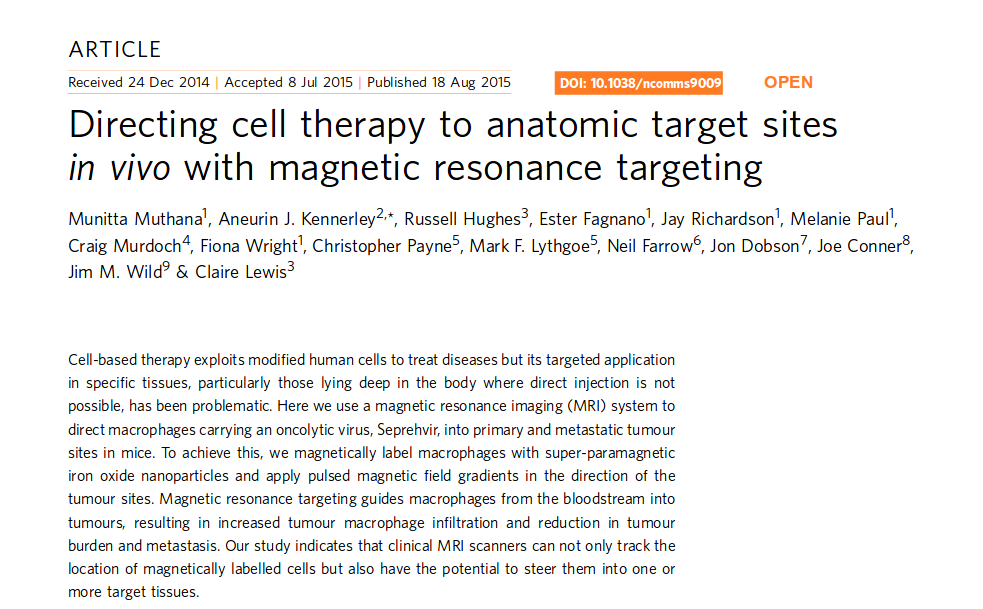
\includegraphics[height=8cm]{cover}
 
\end{frame}



\begin{frame}
 
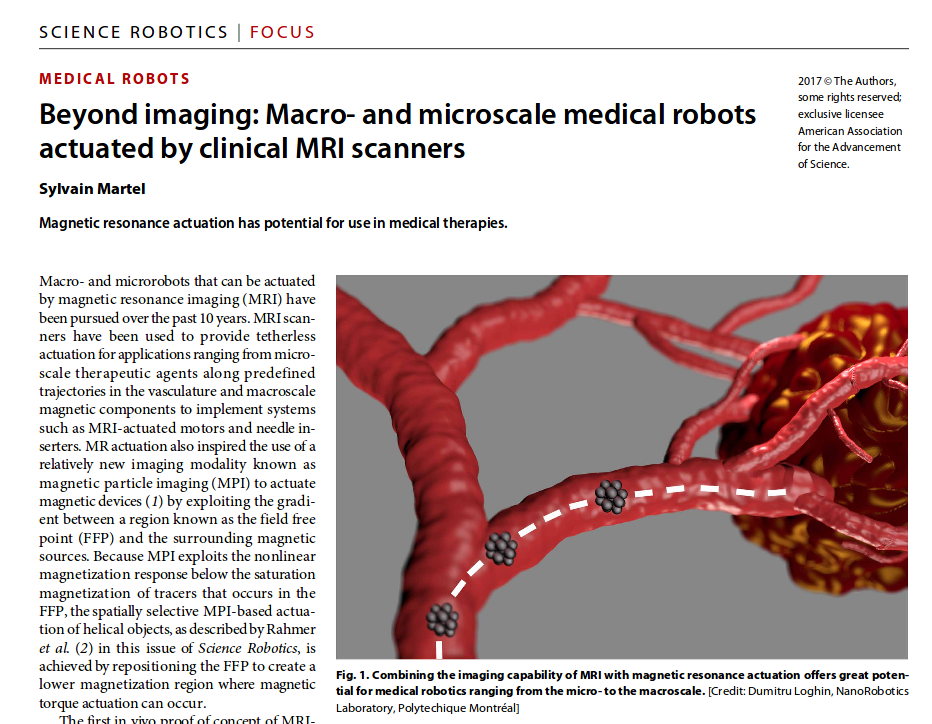
\includegraphics[height=8cm]{mrt_news}
 
\end{frame}

\begin{frame}
\frametitle{Aim: Use MRI to non-invasively steer therapeutic cells to tumors}

% \begin{itemize}
%  \item in vivo (rat)
%  \item prove increased anti-tumour effects
% \end{itemize}


 \begin{figure}
 \centering
 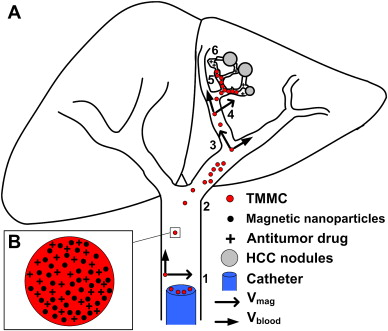
\includegraphics[height=5cm]{steering}
 \end{figure}
 
\end{frame}

\begin{frame}
\frametitle{Cell based Therapy - Overview}

\vspace{-1em}

\begin{columns}

\begin{column}{0.3\textwidth}

Cell therapy = injection of living cells into patient
 
 \vspace{3em}
 
% Cell based therapies can be used to treat various diseases:
% \begin{itemize}
%  \item infarcted myocardium
%  \item spinal cord injury
%  \item cerebral ischaemia
%  \item neurodegenerative diseases (Alzheimer's, Parkinson's)
%  \item cancer
% \end{itemize} 
 
 
\end{column}

\begin{column}{0.7\textwidth}
 \begin{figure}
%  \centering
  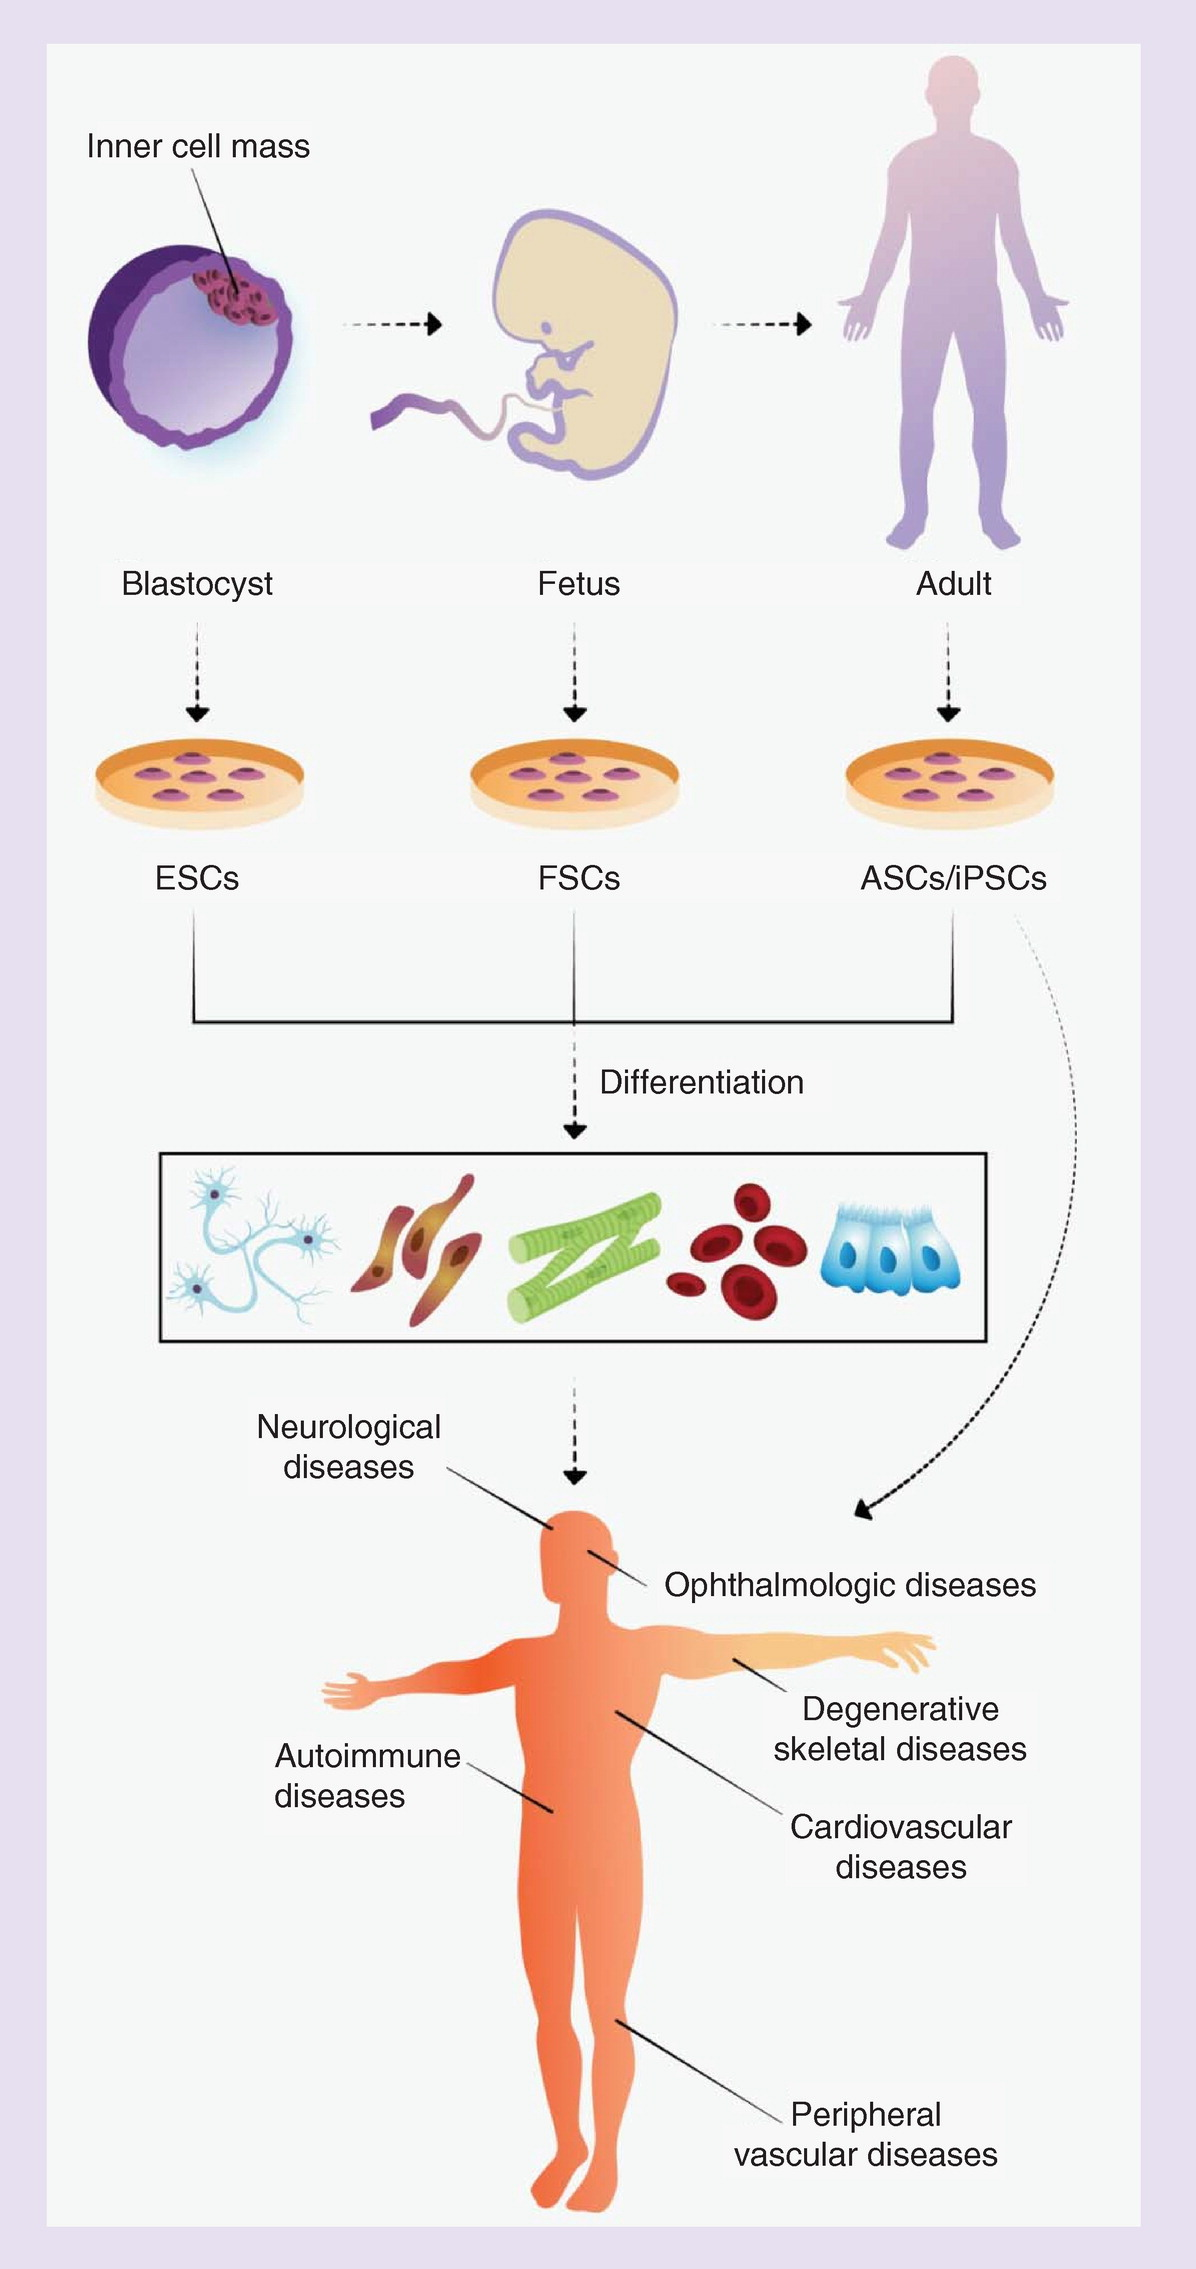
\includegraphics[height=8cm]{cell_therapy_overview}
 \end{figure}

\end{column}
\end{columns}

\end{frame}


% \begin{frame}
% \frametitle{Cell based therapies can be used to treat various diseases}
% 
% 
% \begin{figure}
%  \centering
%  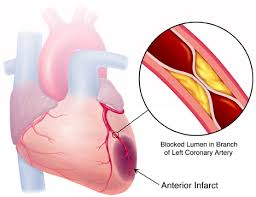
\includegraphics[height=3cm]{infarcted_myocardium} 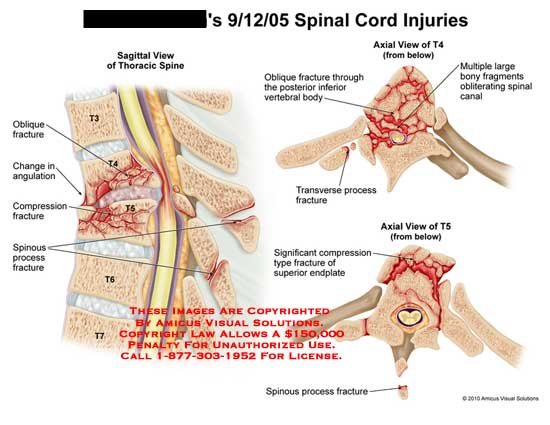
\includegraphics[height=3cm]{spinal_chord_injury} 
%  
% \end{figure}
% 
% 
% \begin{itemize}
%  \item infarcted myocardium
%  \item spinal cord injury
%  \item cerebral ischaemia
%  \item neurodegenerative diseases (Alzheimer's, Parkinson's)
%  \item cancer
% \end{itemize}
% 
% \end{frame}


\begin{frame}
\frametitle{Need to deliver cell-based therapies  \emph{systemically}}
 
\begin{itemize}
 \item disease not confined to one site
 \item tissue inaccessible by direct injection
\end{itemize}
 
 
\begin{figure}
\centering
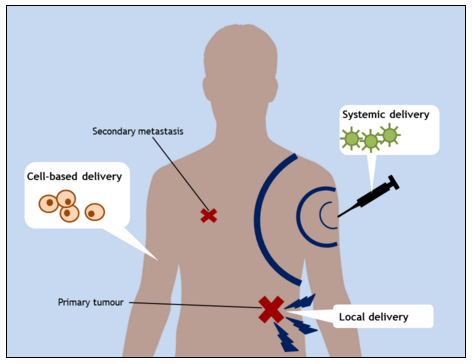
\includegraphics[height=4cm]{systemic}
\end{figure}

 
\end{frame}



\begin{frame}
\frametitle{Therapeutic chemicals lack precise targetting of tumour cells}

\begin{itemize}
 \item reduces therapeutic efficacy
 \item can induce side effects in other body locations: hair loss, nausea, tissue damage
\end{itemize}

\begin{figure}
 \centering
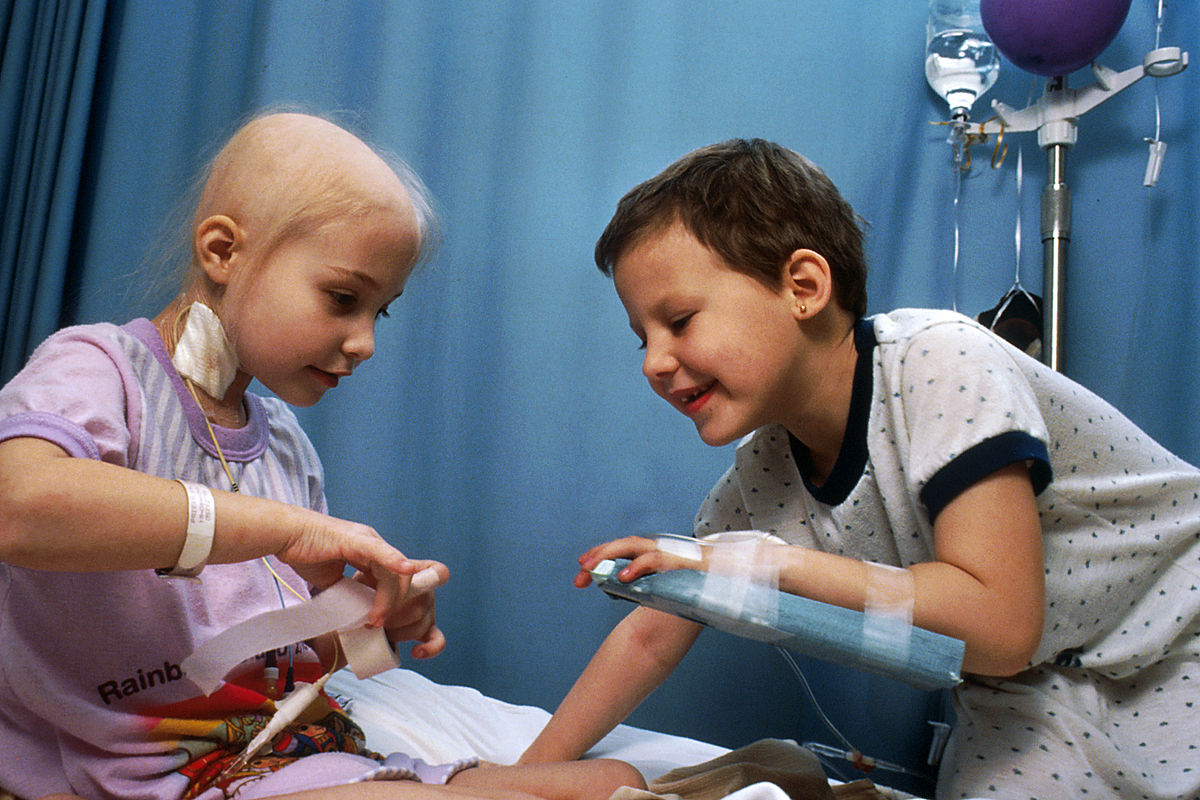
\includegraphics[height=4cm]{hair_loss}
\end{figure}

\begin{itemize}
 \item Current approaches for targetting exploit different properties of tumour cells
  \item Need to find more precise ways to target tumour cells
\end{itemize}

\vspace{1em}




\end{frame}

\begin{frame}
\frametitle{Magnetic Resonance Targetting can increase spatial targetting of tumour cells}

\begin{itemize}
 \item magnetic forces drive macrophages to tumour location
\end{itemize}


\begin{figure}
\centering
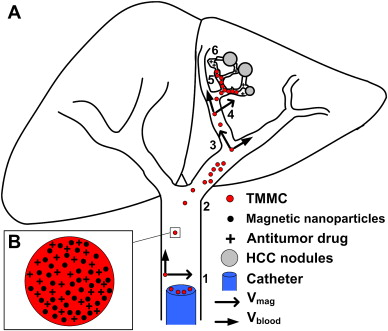
\includegraphics[height=5cm]{steering}
\end{figure}

 
\end{frame}


\begin{frame}
\frametitle{Previous studies used external magnet to attract cells to tumor in rat}


Location - common carotid artery

\begin{figure}
\centering
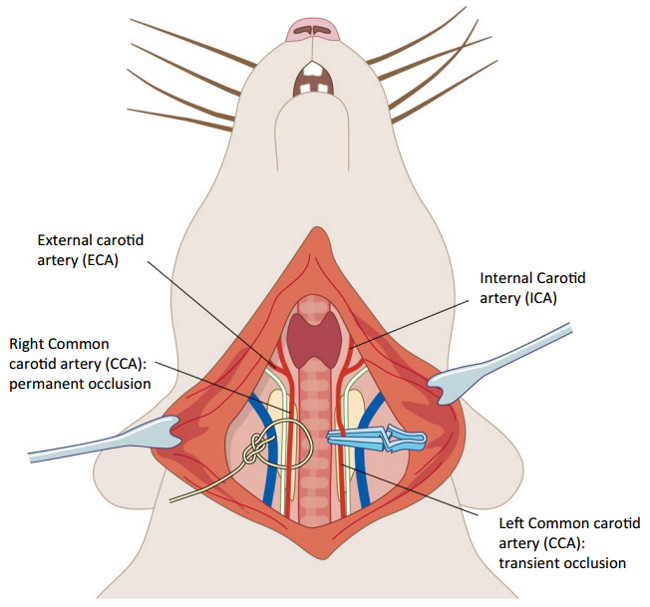
\includegraphics[height=4cm]{rat_cca} 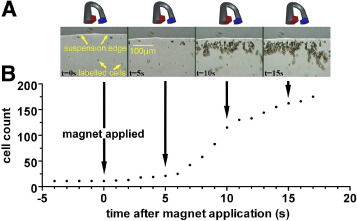
\includegraphics[height=4cm]{external_magnet}\\
Kyrtatos  et al., 2009
\end{figure}

\vfill

But only works for superficial tissues
 
\end{frame}

\begin{frame}
\frametitle{Other study used MRI machines to steer magnetic bead in pigs}

\begin{figure}
\centering
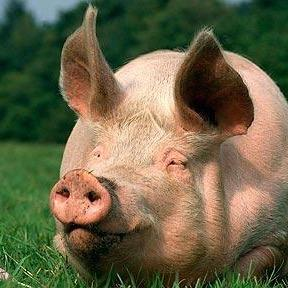
\includegraphics[height=2cm]{pig} 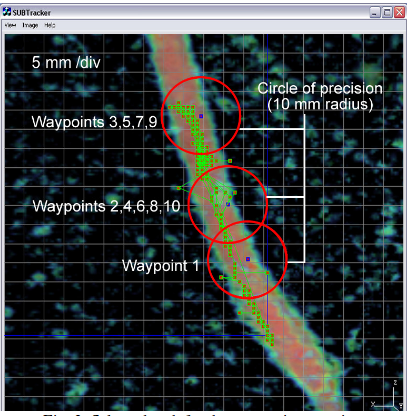
\includegraphics[height=4cm]{pig_tube}\\
A Chanu, Martel S, IEEE Eng Med Biol Soc, 2007
\end{figure}

\vfill

But not attempted using smaller particles such as magnetic induced cells.
 
\end{frame}

\begin{frame}
\frametitle{Aim: Use MRI to non-invasively steer therapeutic cells to tumors}

\begin{itemize}
 \item in vivo (rat) using MR machine
 \item prove increased anti-tumour effects
\end{itemize}


 \begin{figure}
 \centering
 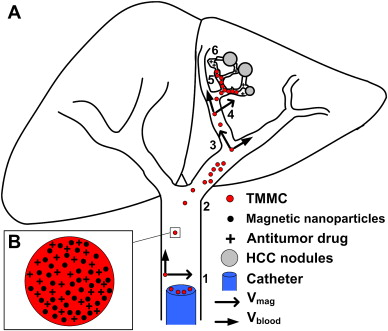
\includegraphics[height=5cm]{steering}
 \end{figure}
 
\end{frame}


\section{Methods}

\begin{frame}
\frametitle{Methods - Magnetic Resonance Targetting of therapeutic cells}
 \begin{figure}
 \centering
 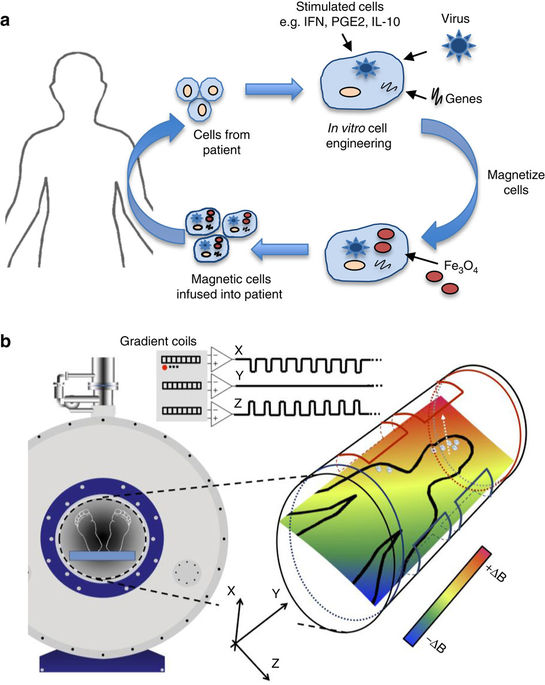
\includegraphics[height=8cm]{mrt_principle}
 \end{figure} 
\end{frame}


\section{Results}

\begin{frame}
\frametitle{In vitro MRT of magnetised particles results in increased uptake in tumor model}
 \begin{figure}
 \centering
 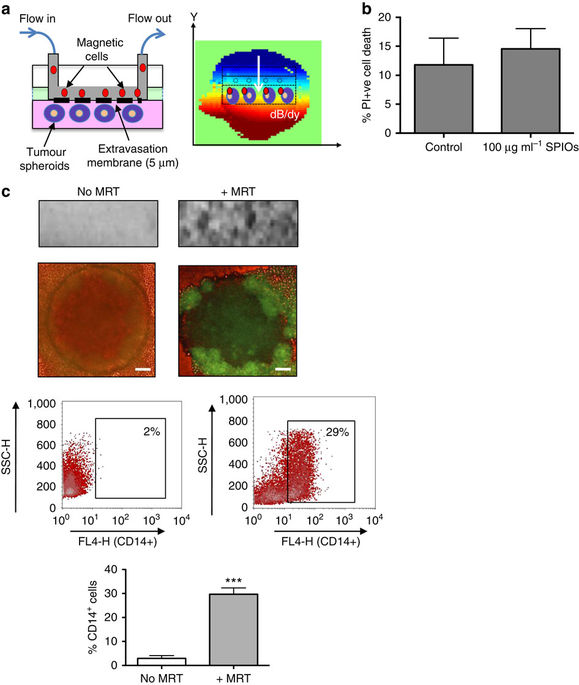
\includegraphics[height=8cm]{muthana_invitro_res}
 \end{figure} 
\end{frame}

\begin{frame}
\frametitle{In vivo MRT leads to increased uptake in tumor areas}
 \begin{figure}
 \centering
 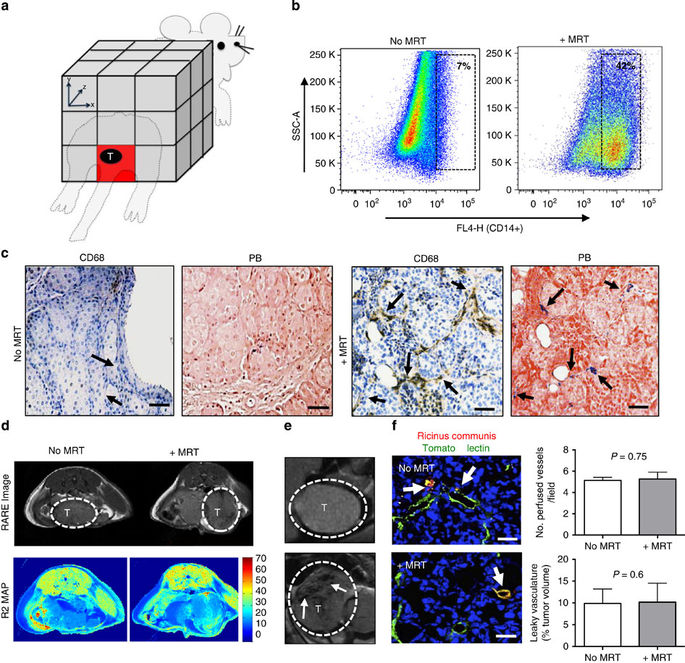
\includegraphics[height=8cm]{muthana_fig2_res}
 \end{figure} 
 
%  \vfill 
 
%  Concern: will MRT affect the vasculature? 
\end{frame}



\begin{frame}
\frametitle{MRT does not affect the vasculature}
 \begin{figure}
 \centering
 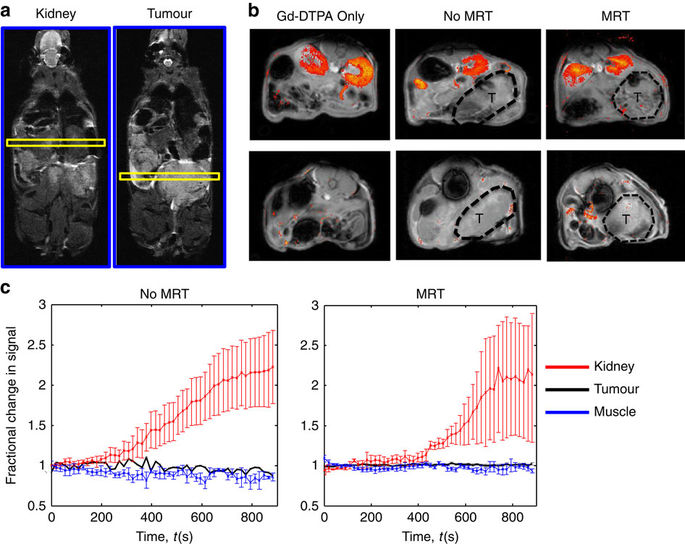
\includegraphics[height=6cm]{muthana_fig3_res}
 \end{figure} 
 
Change in signal in kidney suggests vasculature remained intact
 
\end{frame}

\begin{frame}
\frametitle{MRT can also steer macrophages into lung metastases}
 \begin{figure}
 \centering
 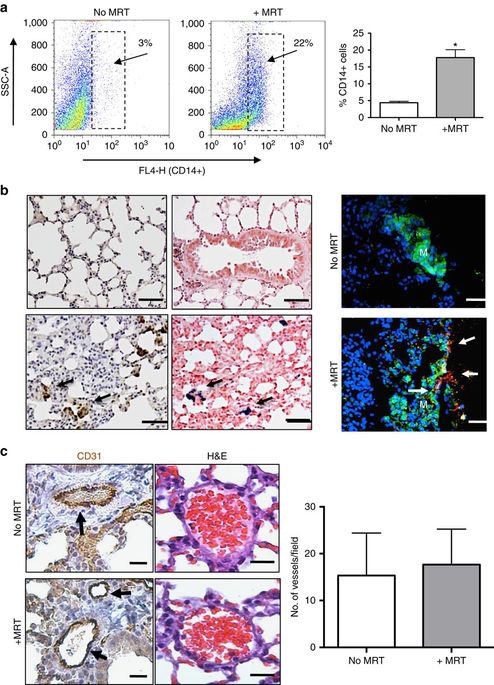
\includegraphics[height=8cm]{muthana_fig4_res}
 \end{figure}
\end{frame}

\begin{frame}
\frametitle{MRT increases anti-tumour effects of macrophages}
 \begin{figure}
 \centering
 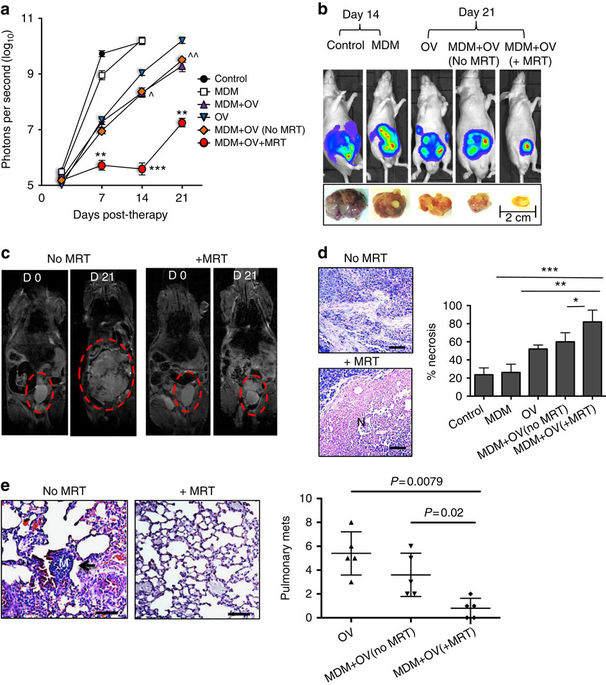
\includegraphics[height=8cm]{muthana_fig5_res}
 \end{figure} 
\end{frame}

\begin{frame}
\frametitle{Discussion}

\textbf{Impact}:
\begin{itemize}
 \item First study to prove MRT \emph{aids treatment of tumours}, in vivo
\end{itemize}

\vfill

\textbf{Limitations}:
\begin{itemize}
 \item MR gradient directions were known a-priori (no imaging required)
\end{itemize}


\end{frame}


\begin{frame}
\frametitle{Subsequent work performs both navigation and imaging simultaneously ...}

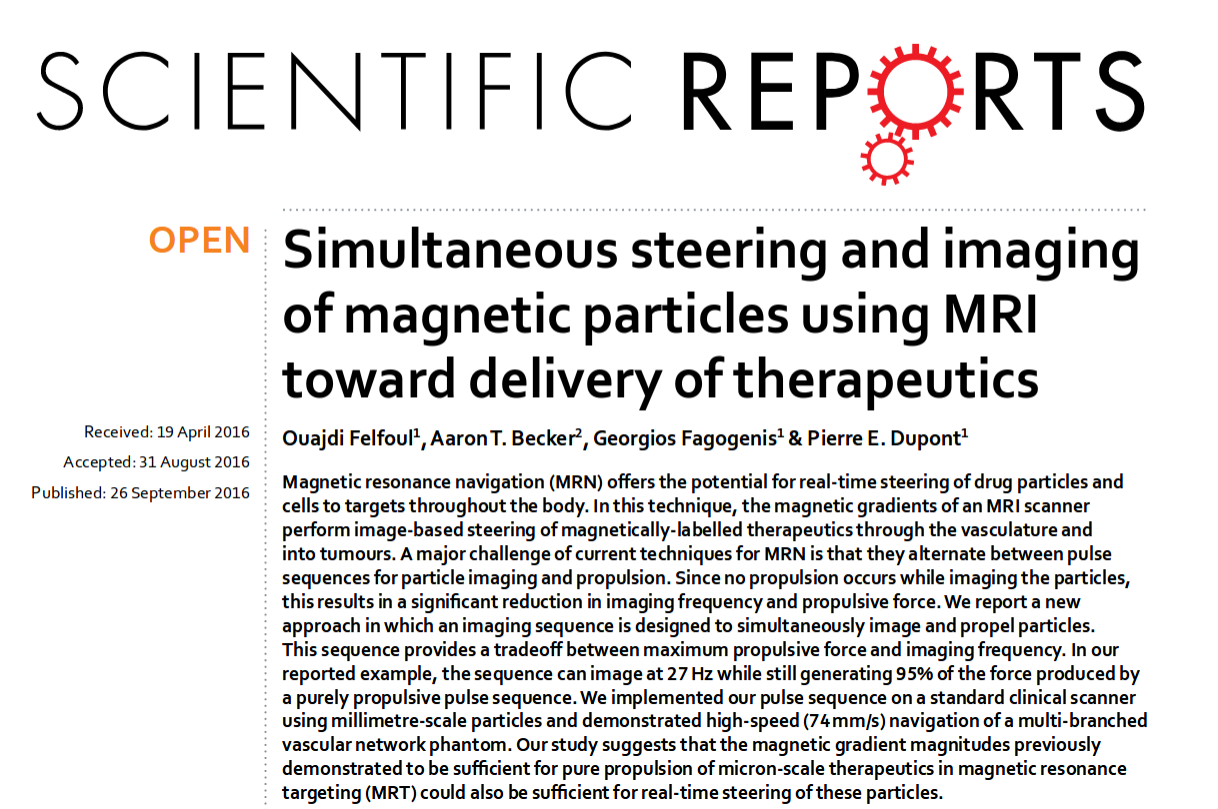
\includegraphics[height=7cm]{simult_mrt_imaging}

\end{frame}


\begin{frame}
\frametitle{... Using specialised MRI sequences}


\begin{figure}
\centering 
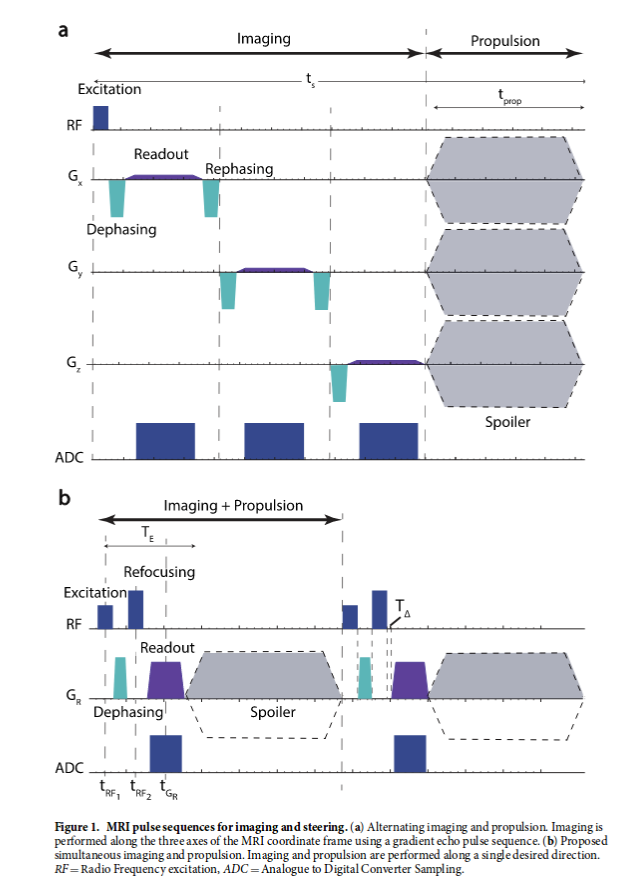
\includegraphics[height=7cm]{propulsion_grads}
\end{figure}


\end{frame}


\begin{frame}
\frametitle{General discussion about MRT}

\textbf{Open questions}:
\begin{itemize}
\item Could it be used to navigate in other body networks?
\item Do MR scans have enough resolution for accurately \emph{mapping} vessel pathways?
\item Same for accurately \emph{navigating} particles through pathway?
\item Do we need to modify current MR scanners to make it work better?
\end{itemize}

\vfill

\textbf{Obstacles in further MRT development}:
\begin{itemize}
 \item restricted access to clinical MR scanners
 \item lack of expertise in robotics community to develop and implement MR sequences
 \item protexted source codes
\end{itemize}




\end{frame}




\end{document}



